%!TEX root = Manuscrit.tex
\chapter{Introduction}
\label{chap:intro}
	\citationChap{[The Computer] was the first machine man built that assisted the power of his brain instead of the strength of his arm.}{Grace Hopper}
	\minitoc
	\newpage


% Début du chapitre
\section{Contexte}

\begin{figure}[h]
	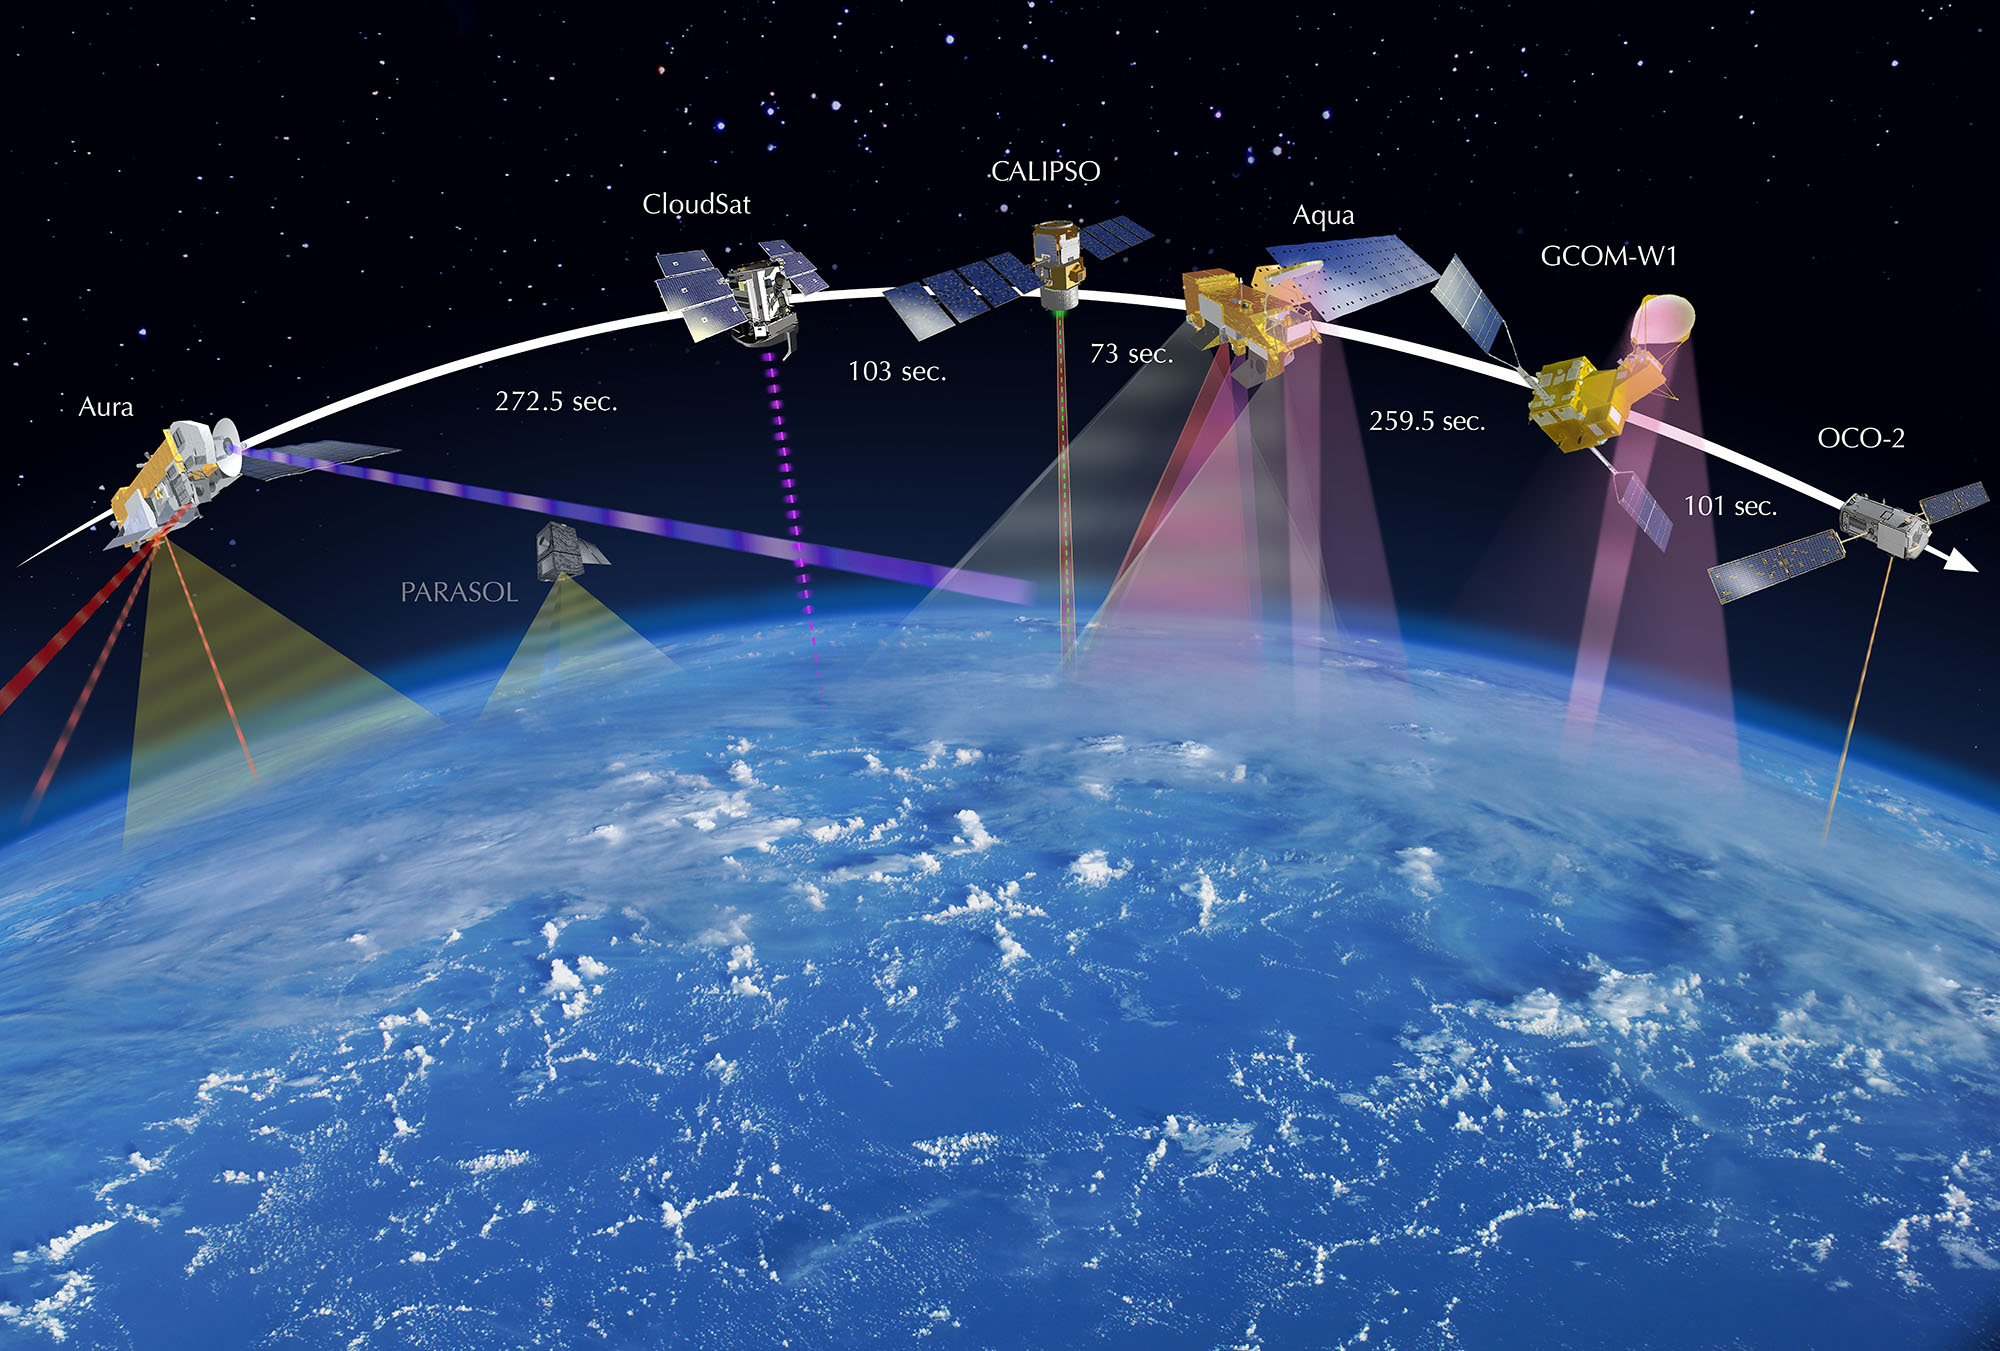
\includegraphics[width=\textwidth]{atrain}
	\caption{Satellites de la constellation A-Train pour l'observation de la Terre en 2018.}
	{\small Crédits image\,: \href{https://commons.wikimedia.org/w/index.php?curid=33645603}{NASA JPL (domaine public)}}
	\label{fig:atrain}
\end{figure}

Toute démarche scientifique débute par une observation. Comprendre un objet passe par un examen attentif des phénomènes qu'il engendre et notre planète ne fait pas exception à cette logique. Ce n'est donc pas une surprise si, lors de l'avènement des premiers programmes spatiaux, les premiers satellites mis en orbite étaient résolument tournés vers la Terre. En effet, l'altitude a permis à la communauté scientifique d'acquérir une toute nouvelle perspective.

L'imagerie aérienne et satellitaire est un outil désormais omniprésent dans les sciences modernes. Comprendre la Terre est un enjeu scientifique majeur, et l'observation est le premier pas nécessaire à toute tentative de modélisation. Qu'il s'agisse de météorologie, d'océanographie, d'écologie ou de géographie, les images de télédétection fournissent une information formidablement riche.

L'intensification des efforts pour imager la Terre dans son intégralité le plus souvent possible n'a donc rien d'étonnant. Des constellations de satellites telles que \gls{Landsat}, \gls{SPOT} ou \gls{Sentinel} survolent chaque semaine l'ensemble du globe. Les satellites Sentinel-2A et 2B acquièrent à eux seuls plus de 6 To de données chaque jour. Pour autant, exploiter cette masse de données n'est pas chose aisée. Interpréter et comprendre une image satellite nécessite une expertise spécifique, mêlant connaissance de la physique du capteur et maîtrise du champ applicatif considéré.

De nombreux domaines peuvent cependant bénéficier de la fouille systématique des données d'observation de la Terre\,:
\begin{itemize}
	\item \textbf{Écologie}\,: études de santé des espaces forestiers (déforestation, pollution), suivi des icebergs et évaluation de la fonte des glaces, détection précoce des dégazages pétroliers et phénomènes de marée noire\dots
	\item \textbf{Météorologie}\,: anticipation et suivi des phénomènes météorologiques intenses (tempêtes, cyclones), évaluation des effets liés au réchauffement climatique\dots
	\item \textbf{Urbanisme}\,: évaluation de l'expansion urbaine et du maillage routier, planification de l'intervention des secours après un séisme, identification des îlots de chaleur\dots
	\item \textbf{Législation}\,: contrôle des lois concernant les cycles agricoles, surveillance de l'apparition de bâti non autorisé, détection de navires de contrebande ou en situation de pêche illégale\dots
\end{itemize}

Malgré leur nombre, les photo-interprètes ne peuvent assumer seuls cette responsabilité. L'automatisation présente alors une alternative intéressante. Conférer aux machines la capacité d'interpréter les images de la Terre permettrait de multiplier les observations, pour en tirer à la fois informations et modèles. Pour ce faire, il convient de s'appuyer sur des outils de perception artificielle adaptés à la compréhension d'images. À l'heure actuelle, l'état de l'art en vision par ordinateur repose majoritairement sur les réseaux de neurones profonds, dont les performances en classification d'images, détection d'objets et reconnaissance de formes ont permis des avancées significatives en intelligence artificielle. Un processus idéal de cartographie itératif pour l'observation de la Terre est détaillé dans la~\cref{fig:workflow}.

Cette thèse s'articule ainsi de la façon suivante. Nous cherchons à concevoir, implémenter et valider des modèles de réseaux de neurones artificiels profonds pour l'interprétation automatisée d'images aériennes et satellites. Ces données peuvent être issues de capteurs multiples, sur une large variété de scènes et pour différents champs d'application.

\begin{figure}[h]
    \centering
    \def\svgwidth{\columnwidth}
    \input{Chapitre1/dessin.pdf_tex}
		\caption{Processus d'interprétation automatique des images d'observation de la Terre pour la cartographie.}
		\label{fig:workflow}
\end{figure}

\section{Domaine}

Cette thèse se place à l'intersection de trois domaines scientifiques\,: la télédétection, la vision artificielle et l'apprentissage statistique. La littérature en vision par ordinateur est abondante concernant l'interprétation de données visuelles, y compris pour la télédétection. Récemment, les méthodes dites d'apprentissage profond ont permis de réaliser des avancées considérables en interprétation automatique d'images. Toutefois, l'essentiel de la communauté s'intéresse aux tâches perceptuelles liées à des scènes de la vie quotidienne. En particulier, les applications s'inscrivent souvent dans le cadre d'extraction d'information dans des images ou vidéos en intérieur ou en extérieur, notamment pour la domotique, la navigation autonome et le multimédia. L'interprétation d'images de télédétection bénéficie de ces recherches, mais ses spécificités en termes de point de vue et de capteurs posent par ailleurs des problèmes nouveaux.

\subsection{Images de télédétection}

Les images de télédétection regroupent une grande variété de données acquises par des moyens spatiaux ou aéroportés. Les observations idéales s'effectuent au nadir, c'est-à-dire à la verticale du sol. En pratique, il est rare que l'instrument de bord soit parfaitement orienté, notamment pour les acquisitions satellitaires. Une étape d'orthorectification est généralement introduite pour corriger les erreurs dues à l'inclinaison de la prise de vue, mais aussi au relief du terrain et aux effets de parallaxe.

Dans tous les cas, les capteurs vont mesurer l'énergie radiative émise par la scène observée. Les capteurs actifs, comme le radar ou le lidar, une onde électromagnétique est envoyée et la mesure porte sur celle renvoyée en retour par la scène. Ils sont ainsi leur propre source de signal. À l'inverse, les capteurs passifs mesurent soit l'énergie radiative émise par la scène (capteurs thermiques dans l'infrarouge), soit l'énergie solaire réfléchie (capteurs multispectraux). Ils nécessitent ainsi une source de lumière externe.

En dépit des spécificités des capteurs, plus nombreux et plus variés que les appareils photos et caméras grand public, le traitement des images de télédétection est proche de celui des images de la vie quotidienne. En effet, dans les deux cas, il s'agit d'extraire de l'information d'images, une tâche de perception artificielle communément appelée vision par ordinateur. Une communauté existe ainsi à la lisière entre télédétection et vision artificielle, concevant ou adaptant des algorithmes de traitement d'images pour l'observation de la Terre.

\subsection{Apprentissage statistique}

La sémantisation des images d'observation de la Terre passe nécessairement par une étape automatisée. En effet, le volume de données acquises chaque année par les capteurs aéroportés et spatiaux est simplement trop conséquent pour que des photo-interprètes humains soient en mesure de les traiter en temps réel.

L'apprentissage statistique permet de déléguer l'extraction de connaissances à une machine afin de l'automatiser. Dans la majorité des cas, il s'agit d'estimer la valeur d'un paramètre ou de prendre une décision parmi un éventail de choix. On parle dans le premier cas de régression et dans le second de classification.

Dans le cas de la photo-interprétation, l'expert humain réalise une étude des images de télédétection à sa disposition pour en réaliser une cartographie. Il s'agit d'un processus de décision, durant lequel le photo-interprète cherche des indices permettant de déclarer qu'un objet ou une région observée appartient à une catégorie précise. L'apprentissage statistique consiste donc à modéliser numériquement ce processus de classification afin de l'automatiser.

Cette modélisation passe par une phase d'apprentissage ou d'entraînement, durant laquelle le modèle consulte des exemples pour alimenter sa base de connaissances. Une fois l'apprentissage terminé, le modèle statistique est alors appliqué sur des données inédites afin de tenter de généraliser les décisions prises sur les exemples. La qualité de cette généralisation est le point critique de cette démarche et peut rencontrer deux types d'obstacle. Si le modèle contient de nombreux paramètres et est exposé à peu d'exemples, alors la base de connaissances risque d'être simplement mémorisée\,: on parle alors de surapprentissage. Inversement, si le modèle apprend sur de nombreux exemples mais avec trop peu de paramètres, il ne sera pas en mesure d'approcher efficacement la fonction de décision. Il s'agit ainsi de trouver des modèles capables d'exploiter au mieux l'ensemble de leurs paramètres pour tirer profit de l'ensemble des exemples d'apprentissage disponibles.

L'émergence de l'apprentissage profond dans les années 2000 a fortement contribué à renouveler la littérature en apprentissage statistique. En particulier, les réseaux de neurones profonds, bien que théorisés et mis en application dès les années 1960, ont trouvé une résonance particulière avec l'ère des données massives. Les grandes bases de données d'apprentissage, combinées avec des modèles de réseaux de neurones artificiels profonds et des implémentations parallèles permettant de rendre les calculs traitables en temps raisonnable, ont permis d'importantes avancées en perception artificielle. Le traitement d'images a notamment largement bénéficié de cette conjonction. Dès 2012, les réseaux de neurones convolutifs profonds se sont imposés comme le nouvel état de l'art pour la classification d'images et ont petit à petit conquis une grande partie des tâches de perception visuelle.

\subsection{Vision par ordinateur}

La vision par ordinateur regroupe l'ensemble des techniques conçues pour l'interprétation automatisée des images. Dès les années 60, les experts en intelligence artificielle se sont penchés sur la possibilité de simuler les capacités sensorielles humaines. La vision étant le sens humain le plus mis à contribution, il est naturel que les travaux en ce sens aient été nombreux. La démocratisation des appareils photos et caméras numériques a d'autant plus accéléré les possibilités offertes en traitement d'images, non seulement grâce aux traitements correcteurs embarqués au sein-même des capteurs, mais également par la facilité nouvelle du post-traitement sur ordinateur.

Le Graal de la vision par ordinateur consiste à émuler la capacité du cerveau humain à interpréter une scène dynamique à partir des signaux visuels, en particulier à identifier rapidement les objets et à anticiper leurs mouvements. Ces fonctions cognitives sont indispensables pour la navigation autonome en robotique, mais bénéficient également aux applications en fouille de données. La numérisation automatique de documents anciens, la recherche en ligne d'images similaires ou l'audio-description automatique sont autant d'exemples de tâches pouvant s'appuyer sur une brique d'interprétation d'images.

En particulier, les efforts de la communauté de la vision par ordinateur se sont concentrés sur la reconnaissance d'objets dans des images, incluant à la fois leur identification et leur localisation. De nombreux descripteurs \emph{ad hoc} ont été introduits pour des applications aussi variées que la détection de visages, la classification automatique de photographies d'espèces animales ou la reconnaissance optique de caractères. Le dénominateur commun de ces travaux est de chercher à donner du sens aux images. Extraire la sémantique d'une information visuelle non structurée est également l'objectif de l'observation de la Terre.
Lidar
Cette thèse se trouve ainsi au croisement entre la télédétection, la vision par ordinateur et l'apprentissage automatique. En particulier, nous nous proposons de mettre en \oe{}uvre des méthodes d'apprentissage profond pour l'interprétation automatique d'images d'observation de la Terre.

\section{Problématique}

L'objectif de cette thèse est de proposer des méthodes d'apprentissage profond permettant de cartographier automatiquement la Terre en tirant profit des grandes quantités d'images acquises chaque jour. En particulier, il s'agit de sémantiser les images sous formes de cartes thématiques, notamment pour l'occupation des sols. Plusieurs questions découlent de cet objectif\,:
\begin{itemize}
	\item Quels outils mettre en \oe{}uvre pour la cartographie automatique à partir d'images d'observation de la Terre ?
	\item Comment exploiter les multiples capteurs multispectraux, hyperspectraux et Lidar dans un cadre d'apprentissage profond ?
	\item Peut-on mettre à profit la revisite d'une même zone par plusieurs instruments pour enrichir les informations géographiques ?
	\item À quel point les modèles statistiques supervisés peuvent-ils s'appliquer à large échelle, pour cartographier l'intégralité de la planète ?
	\item Est-il possible d'extraire des images une information spatialement structurée pouvant renseigner sur la nature des objets et leur agencement géographique ?
\end{itemize}

En premier lieu, les outils pour l'interprétation automatique d'images sont légion. Si les réseaux de neurones artificiels sont populaires dans l'état de l'art pour la vision par ordinateur, leurs succès sont récents et leur introduction pour la télédétection est encore nouvelle. Il sera donc nécessaire dans un premier temps d'étudier le comportement des réseaux convolutifs profonds par rapport aux approches de l'état de l'art en classification d'images de télédétection. Le~\cref{chap:etat} est l'occasion de rappeler les fondamentaux théoriques de l'apprentissage profond, et plus particulièrement des réseaux de neurones convolutifs ainsi que leurs applications en perception artificielle. Le~\cref{chap:cartographie} démontre les limites du paradigme de classification par région dans le cadre de la cartographie automatisée d'images aériennes et de met en avant la pertinence des réseaux entièrement convolutifs sur cette tâche.

Cependant, comme nous l'avons vu précédemment, les dispositifs d'observation de la Terre couvrent des domaines de longueur d'onde bien différents des appareils photographiques habituels. En outre, les capteurs optiques sont parfois complétés par des appareils Lidar qu'il est nécessaire de savoir exploiter pour interpréter les images de télédétection le plus fidèlement possible. En effet, l'observation de la Terre passe couramment par l'acquisition de données complémentaires sur une même zone à partir de capteurs hétérogènes. Qui plus est, les nouvelles bases de données géographiques libres d'accès représentent une source de données inédite encore inexploitée. La possibilité de fusionner ces données afin de tirer profit des avantages de chaque capteur serait donc un atout majeur en cartographie. Par conséquent, le~\cref{chap:extension} étendra ainsi les résultats obtenus sur des images \glsfirst{RVB} à l'ensemble des données issues d'appareils multispectraux et hyperspectraux, ainsi qu'aux modèles de terrains dérivés des acquisitions \glsfirst{Lidar}. Le~\cref{chap:multimodal} introduit par la suite différentes stratégies d'apprentissage multi-modal pour les réseaux profonds afin de répondre à la problématique de fusion de données, aussi bien dans le cas multi-capteurs que pour la prise en compte de connaissances \emph{a priori}.

La généralisation des modèles statistiques étant par ailleurs l'élément fondamental permettant de passer à l'échelle, il est nécessaire d'étudier la capacité de généralisation des réseaux profonds sur de grands jeux de données comportant une large variété de scènes. En effet, cartographier l'intégralité de la surface du globe nécessite une robustesse du modèle aux variations locales de la biosphère, qu'elles soient spatiales ou temporelles. Notamment, l'apprentissage supervisé n'est parfois possible que sur des jeux de données de petite taille, à partir desquels il n'est pas trivial de construire des modèles généralistes. Le~\cref{chap:generalisation} s'intéresse à ces deux problèmes.

Enfin, si l'interprétation d'images de télédétection permet de construire des cartes thématiques, c'est bien souvent les relations entre les sous-parties de ces cartes qui sont intéressantes. En particulier, l'analyse niveau objet est une approche incontournable en géographie, car elle seule permet de modéliser les structures et leur agencement. Le~\cref{chap:structure} explore donc différentes possibilités pour donner une structure spatiale aux cartes produites par les modèles de classification dense pixel à pixel proposés jusqu'ici.

Le~\cref{chap:conclusion} clôt ce manuscrit et discute des pistes de recherches futures envisageables à la suite de ces travaux.

\section{Contributions}

Cette thèse apporte 4 contributions majeures.
\begin{enumerate}
  \item Elle participe à établir les réseaux de neurones convolutifs comme nouvel état de l'art pour la cartographie automatisée d'images de télédétection.
  \item Elle démontre la possibilité d'étendre les domaines d'application desdits réseaux à l'ensemble des capteurs optiques usuels.
  \item Elle montre qu'il est possible et pertinent d'utiliser les informations présentes dans plusieurs capteurs lorsque c'est possible.
  \item Elle montre que ces approches ne se confinent pas à des cas spécifiques, mais peuvent s'étendre à l'ensemble du globe.
\end{enumerate}

Ces travaux ont fait l'objet de plusieurs publications\,:

\subsubsection*{Publications en revues internationales à comité de lecture}

\fullcite{audebert_segment-before-detect_2017}

\fullcite{audebert_beyond_2017}

\subsubsection*{Publications en conférences internationales à comité de lecture}

\fullcite{audebert_how_2016}

\fullcite{audebert_semantic_2016}

\fullcite{audebert_fusion_2017}

\fullcite{audebert_joint_2017}

\fullcite{audebert_generative_2018}

\medskip



%\bibliographystyle{francaissc}
%\bibliography{Chapitre1/Self}
\printbibliography
